
%(BEGIN_QUESTION)
% Copyright 2010, Tony R. Kuphaldt, released under the Creative Commons Attribution License (v 1.0)
% This means you may do almost anything with this work of mine, so long as you give me proper credit

Suppose we have a Koyo ``CLICK'' PLC connected to three pushbutton switches as shown in this illustration:

$$\includegraphics[width=15.5cm]{i04666x01.eps}$$

Determine the switch actuation statuses (i.e. pressed versus released) given the ``live'' display of the ladder logic program shown here:

$$\includegraphics[width=15.5cm]{i04666x02.eps}$$

Also, determine the status of the lamp connected to the PLC's {\tt Y1} output.

\underbar{file i04666}
%(END_QUESTION)





%(BEGIN_ANSWER)

Switch statuses:

\begin{itemize}
\item{} Switch A = {\bf pressed}
\item{} Switch B = {\bf released}
\item{} Switch C = {\bf released}
\end{itemize}

The lamp will be de-energized.

%(END_ANSWER)





%(BEGIN_NOTES)


%INDEX% PLC, relating I/O status to virtual elements 

%(END_NOTES)


